\newpage
\section{Efficiently solvable abstrations}

\begin{displayquote}
  \textit{Abstraction for efficient optimisation.}
\end{displayquote}

In optimisation for supervised learning we know that;
linear models can be solved analytically,
convex problems converge quickly.
What makes an RL problem easy to solve? Is there linearity or convexity
within RL problems that we can use to find solutions more efficiently?

% bellman eqn is hard to solve (how hard?)
% Existing solvers of MDPs such as are not efficient: value iteration requires at
% least \href{https://en.wikipedia.org/wiki/EXPTIME}{EXPTIME} iterations,
% policy iteration requires ???, or policy gradients,
% require a ??? amount of computation.
% Yet, recent work \cite{} has shown that MDPs require at least $\Omega(|S|^2|A|).$

While some interesting work has been done exploring convex RL \cite{ODonoghue2012a, Barratt2019},
we chose to look into linear RL.

\subsection{Linear Markov decision problems (LMDPs)}

\begin{displayquote}
\textit{Why linear MDPs?}
\end{displayquote}

% How are we exploiting linearity?
% Linearisation around the optima? Intuition. How to see this? Stephen!?
% Intuition.

% \subsubsection{Existing linear methods}
%
% The optimal policy of a MDPs can be found be using linear programming.
% Traversing through the (value ??) space, ...?

% many mathematical tools for analysis.
% we know linear systems can be solved efficiently.

Linear systems are easy to solve. (ref). They have $\mathcal O(n^3)$ complexity.

Imagine if your life were linear, in the sense of effort and achieving goals.
More work in equals proportionally more rewards. This makes decision making
a lot more simple. Pick the most rewarding ???, and work hard.

Saxe el al. observe the power of linearity: \textit{"Consider two standard MDPs
$M_1 = \{S, A, P, R_1\}$ and $M_2 = \{S, A, P, R_2\}$ which have
identical state spaces, action sets, and transition dynamics but differ in their
instantaneous rewards $R_1$ and $R_2$. These may be solved independently to
yield value functions $V_1$ and $V_2$. [If the problems were linear then] the value function of the MDP
$M_{1+2} = \{S, A, P, R_1 +R_2\}$, whose instantaneous rewards are the sum of the
first two, [would be] $V_{1+2} = V_1 + V_2$.} \cite{Saxea}

% why do we care about multitask!?
The ability to recycle knowledge from a task to a new task is !!!



% are there other famous examples of linearising something to make it easy to solve?!?

\subsubsection{What do we mean by a linear MDP?}

Do we mean that the value function is a linear function of the policies,
of the reward function, of the transition function? Others have tried to incorporate
linearity into MDPs in a few different ways.

\begin{itemize}
  \tightlist
  \item Todorov constructs a linearised MDP that is linear in the 'control' (a proxy for the policy). \cite{Todorov2006}
  \item Jin et al. construct a MDP where the value is a linear function of a state-action representation and of a policy embedding. \cite{Wang}
  \item Levine et al. contstruct a learner that assumes a linear transition function, allowing the use of \href{https://en.wikipedia.org/wiki/Linear%E2%80%93quadratic_regulator}{LQR} solvers.\cite{Levine2019}
  \item Pires et al. construct a factored linear MDP that allows the TD operator to be applied in a lower dimensional space. \cite{Pires2016}
\end{itemize}

Todorov's formulation appears to be the most powerful. By having a linear
relationship between the value and the control, we can easily search for controls that
are optimal. For the rest of this work we will refer to these as LMDPs.

\subsubsection{Constructing a linear MDP}

\begin{figure}[h!]
  \centering
  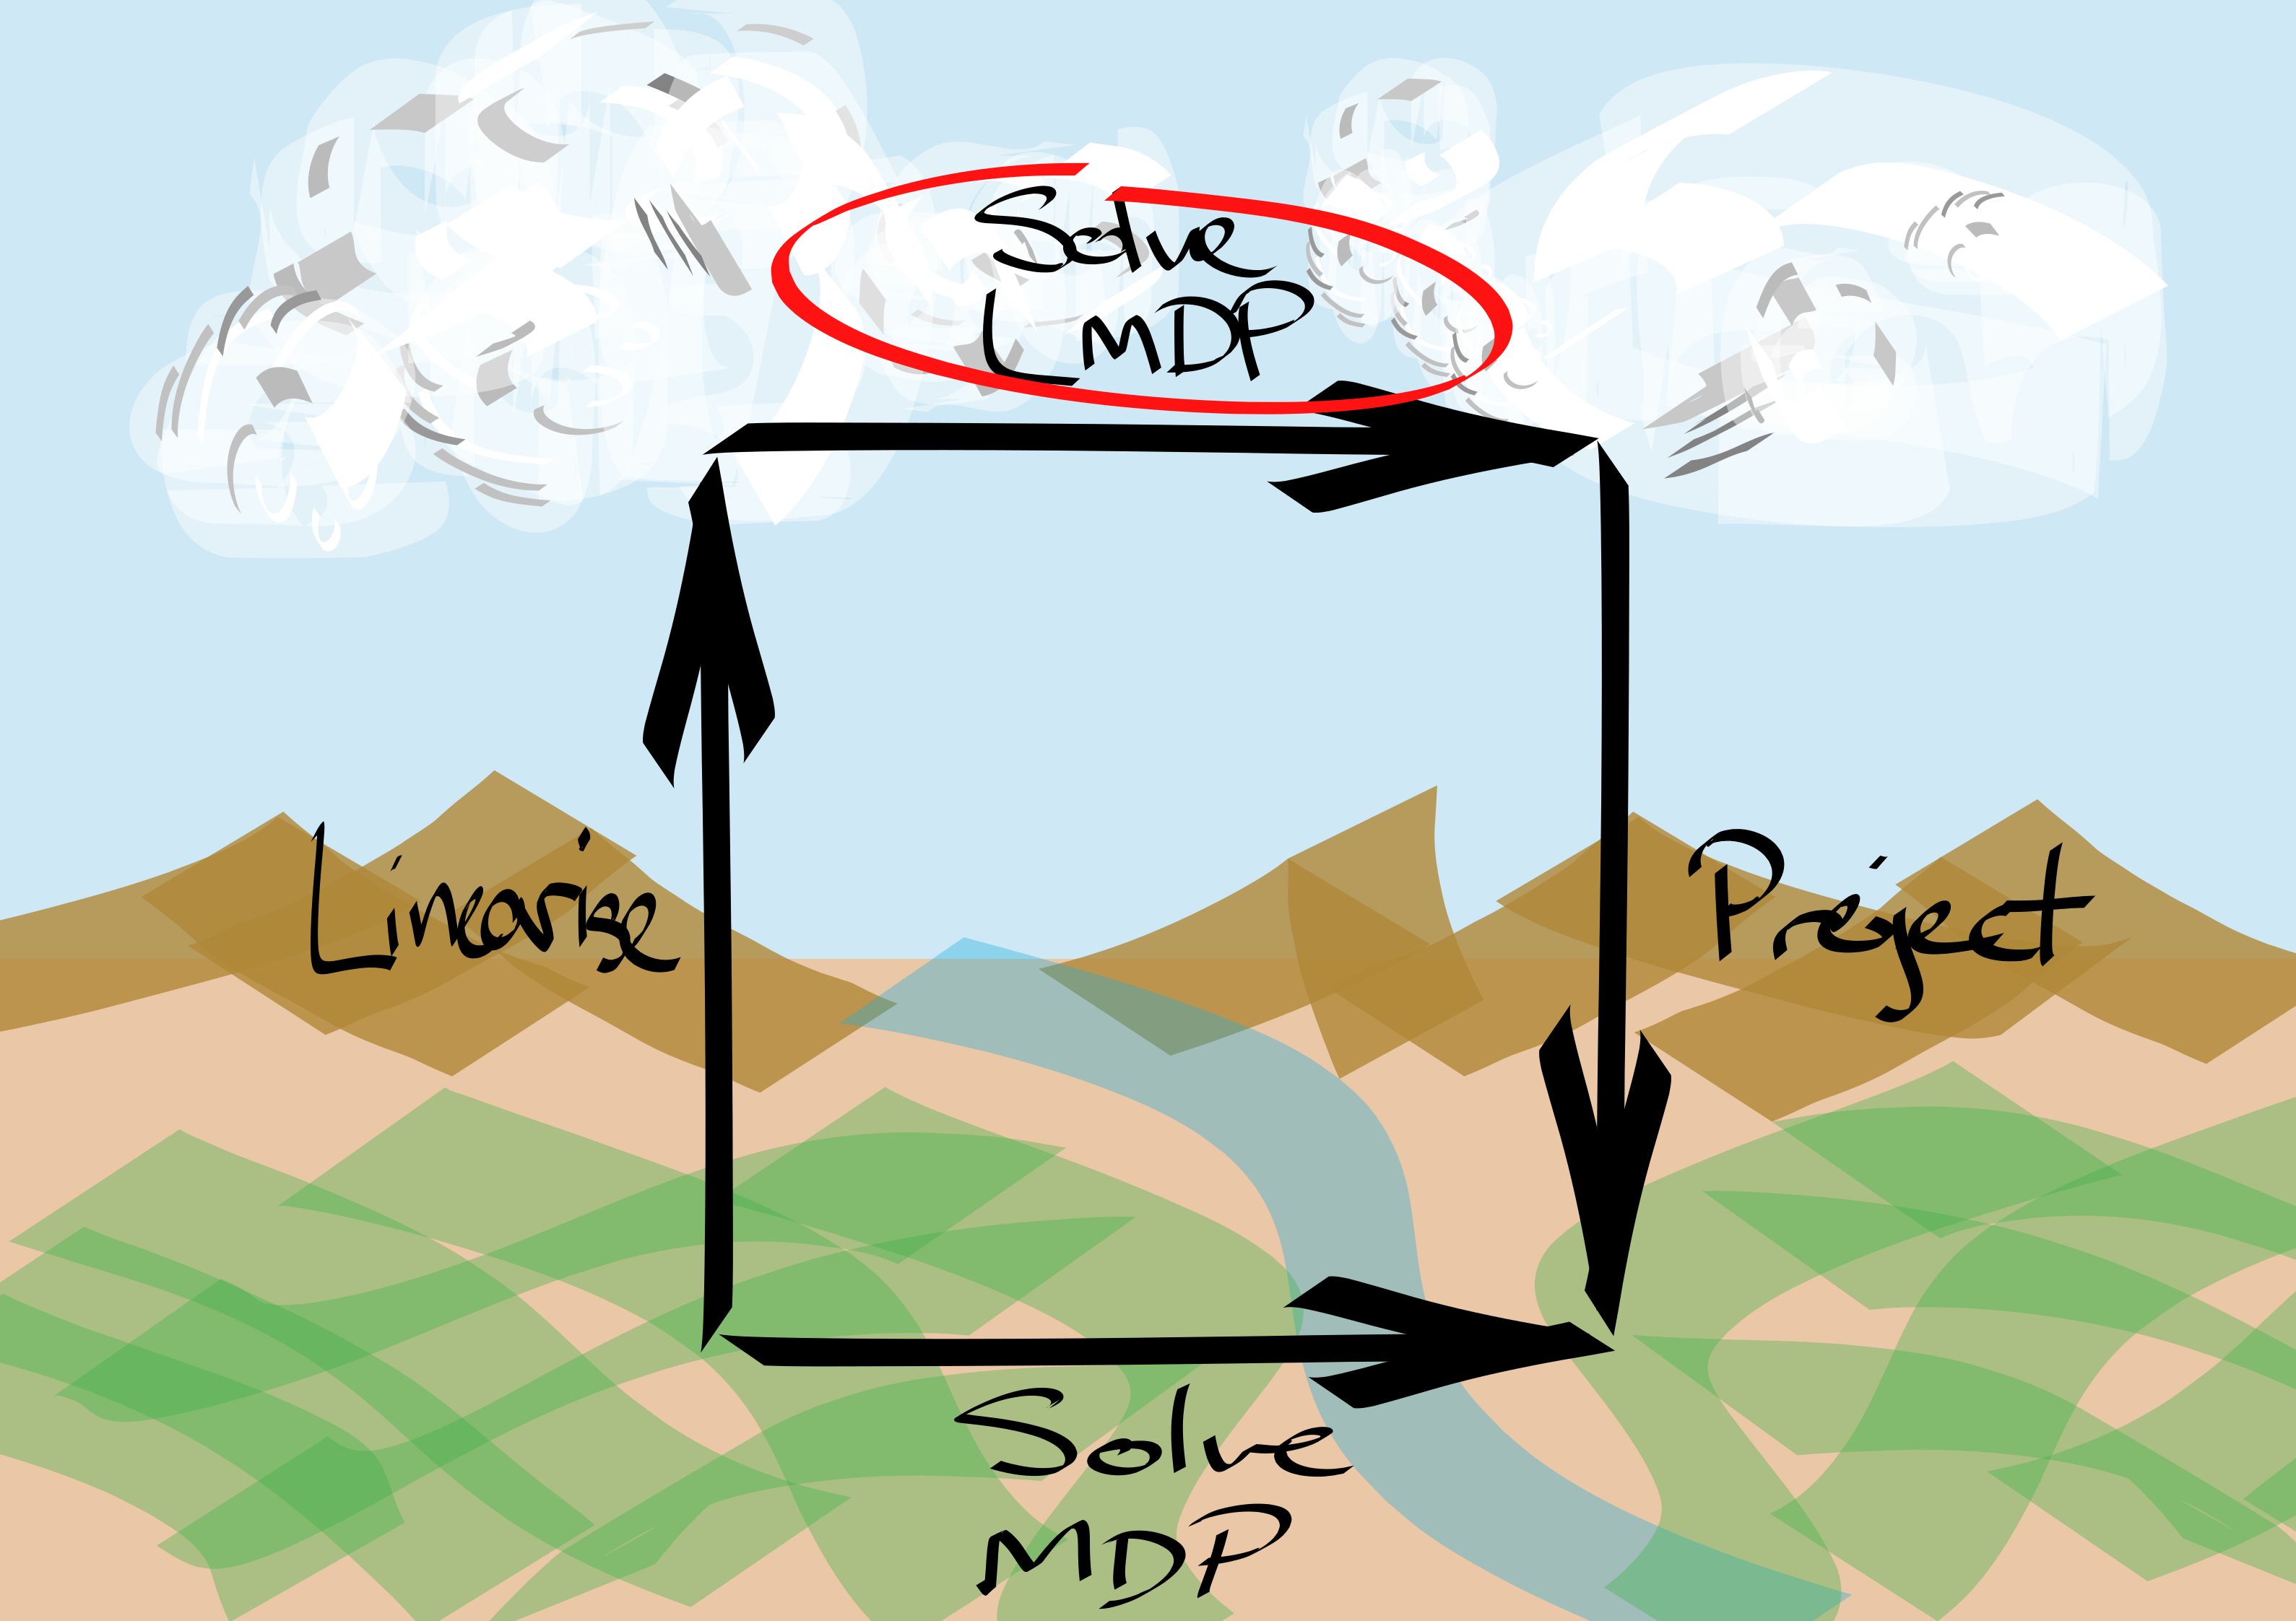
\includegraphics[width=0.6\textwidth,height=0.3\textheight]{../../pictures/drawings/abstract-representations-solve.png}
  \caption{'Solving the LMDP'}
\end{figure}

To build a LMDP that acts similarly to a MDP, Todorov \cite{Todorov2006} uses a few main {\color{red}tricks};

\begin{itemize}
\tightlist
  \item
  they allow the agent to pick actions in the space of possible transitions, which they name controls, $u: S \to S$, rather than the action space.
  \item
  to ensure that chosen controls are possible under the given transition function, a new reward is added.
  Controls are rewarded if they are close to the 'unconstrained dynamics', $p(s' | s)$.
  \item
  rather than maximizing the cumulative reward, we maximise the exponentiated cumulative rewards.
  $\mathop{\text{max}}_{\pi} \mathop{\mathbb E}_{\zeta \sim D(\pi)} e^{R(\zeta)}$ \cite{EricWarrenFox2016}
\end{itemize}

The intuition behind these tricks seems to be; we have allowed the learner to pick an arbitrary control.
This simplifies the optimisation problem. But, now the learner might pick a control that is not possible
under the given transition function. So we incentivise controls that are close to the underlying dynamics.
\textit{"It is reminicent of a linear programming relaxation in integer programming"} \cite{Todorov2009}.

% What is the relationship to other action embedding strategies? {\color{red}!!!!!}

% Why did they need these tricks? Which ones were necessary / sufficient? !!!!!!!

% formal definition
Putting these tricks together, a linear markov decision process can be formulated as;
LMDP = $\{S, U, p, q, \gamma\}$. Where $S$ is the state space, $U$ is the space of possible controls (aka any transition function),
$p: S \to S$ is the unconditioned dynamics, and $q \in \mathbb R^{|S|}$ is state rewards.
Our goal is to find the control, $u: S \to S$, that gvies the highest exponentiated cumlative reward $z \in \mathbb R_+^{|S|}$.

\begin{align}
\log z_{u^{* }}(s) &= \mathop{\text{max}}_{u} q(s) - \text{KL}(u(\cdot| s) \parallel p(\cdot | s)) + \gamma \mathop{\mathbb E}_{s' \sim u(\cdot | s)} \log z_{u^{* }}(s') \tag{1}\\
u^{* }(\cdot | s) &= \frac{p(\cdot | s)\cdot z_{u^{* }}(\cdot)^{\gamma}}{\sum_{s'} p(s' | s) z_{u^{* }}(s')^{\gamma}} \tag{2}\\
z_{u^{* }} &= e^{q(s)}\cdot P z_{u^{* }}^{\gamma} \tag{3}
\end{align}

By definition, a linearised Bellman equation can be constructed (1). After some algebra,
it can be shown that the optimal policy has the form in (2).
And! We can solve for the value of this policy (aka we can find the optimal policy)
by solving the linear equation in (3). (see appendix [] for further explanation and a derivation)

\begin{displayquote}
\textit{Let's try and understand this linear MDP we have constructed.}
\end{displayquote}

\subsubsection{\color{red}The unconstrained dynamics and state rewards}

Initially, I thought of the unconstrained dynamics as the expected result of using random policy
$p(s' | s) = \int_a P(s' | s, a)U(a|s)$, a random walk using the transition function.
However, while this make sense intuitively, it turns out to be wrong.

Rather than state-action rewards $r: S \times A \to \mathbb R$, we have state rewards $q: S \to \mathbb R$.
How can state rewards direct behaviour? They can't, and they can. State rewards are not capable of giving rewards for actions taken.
Rather, the action dependent part of the reward is captured by the KL divergence between the control and the unconstrained dynamics.
So the unconstrained dynamics are responsible for rewarding actions.
But, states with higher state reward will be perferable.

\subsubsection{The optimal policy}

What should we make of the form of the optimal control?

\begin{align*}
u^{* }(\cdot | s) &= \frac{p(\cdot | s)\cdot z_{u^{* }}(\cdot)^{\gamma}}{\sum_{s'} p(s' | s) z_{u^{* }}(s')^{\gamma}}
\end{align*}

So the optimal control is the one that transitions to a new state with a
probability proportional to the discounted exponentiated value of that state.
That seems sensible, and is closely realted to a common way (refs...) of constructing a policy from $Q$ values.

\begin{align*}
\pi(\cdot|s) = \sigma(\tilde Q(s, \cdot))
\end{align*}

Where $\tilde Q$ is an estimate of the state action values, maybe from SARSA or Q-learning.
And $\sigma$ is the softmax operator.

\subsubsection{Solving for the optimal value}

What should we make of the form of the value estimate?

\begin{align*}
z_{u^{* }} &= e^{q(s)}\cdot P z_{u^{* }}^{\gamma}
\end{align*}

In the undiscounted case (aka first exit case), where $\gamma=1$, this turns
into an eigen value problem $z = QPz = Az$.
$A$ is positive semi definite bc ...

Has nice convergence properties because it is contractive.

Converges to the eigenvector of QP, with eigen value being prop to...
Amount $QP$ expands and amount $/gamma$ contracts.

{\color{red}TODO. although, how necessary is this!?}

\subsection{Solving a MDP}

\begin{figure}[h!]
\centering
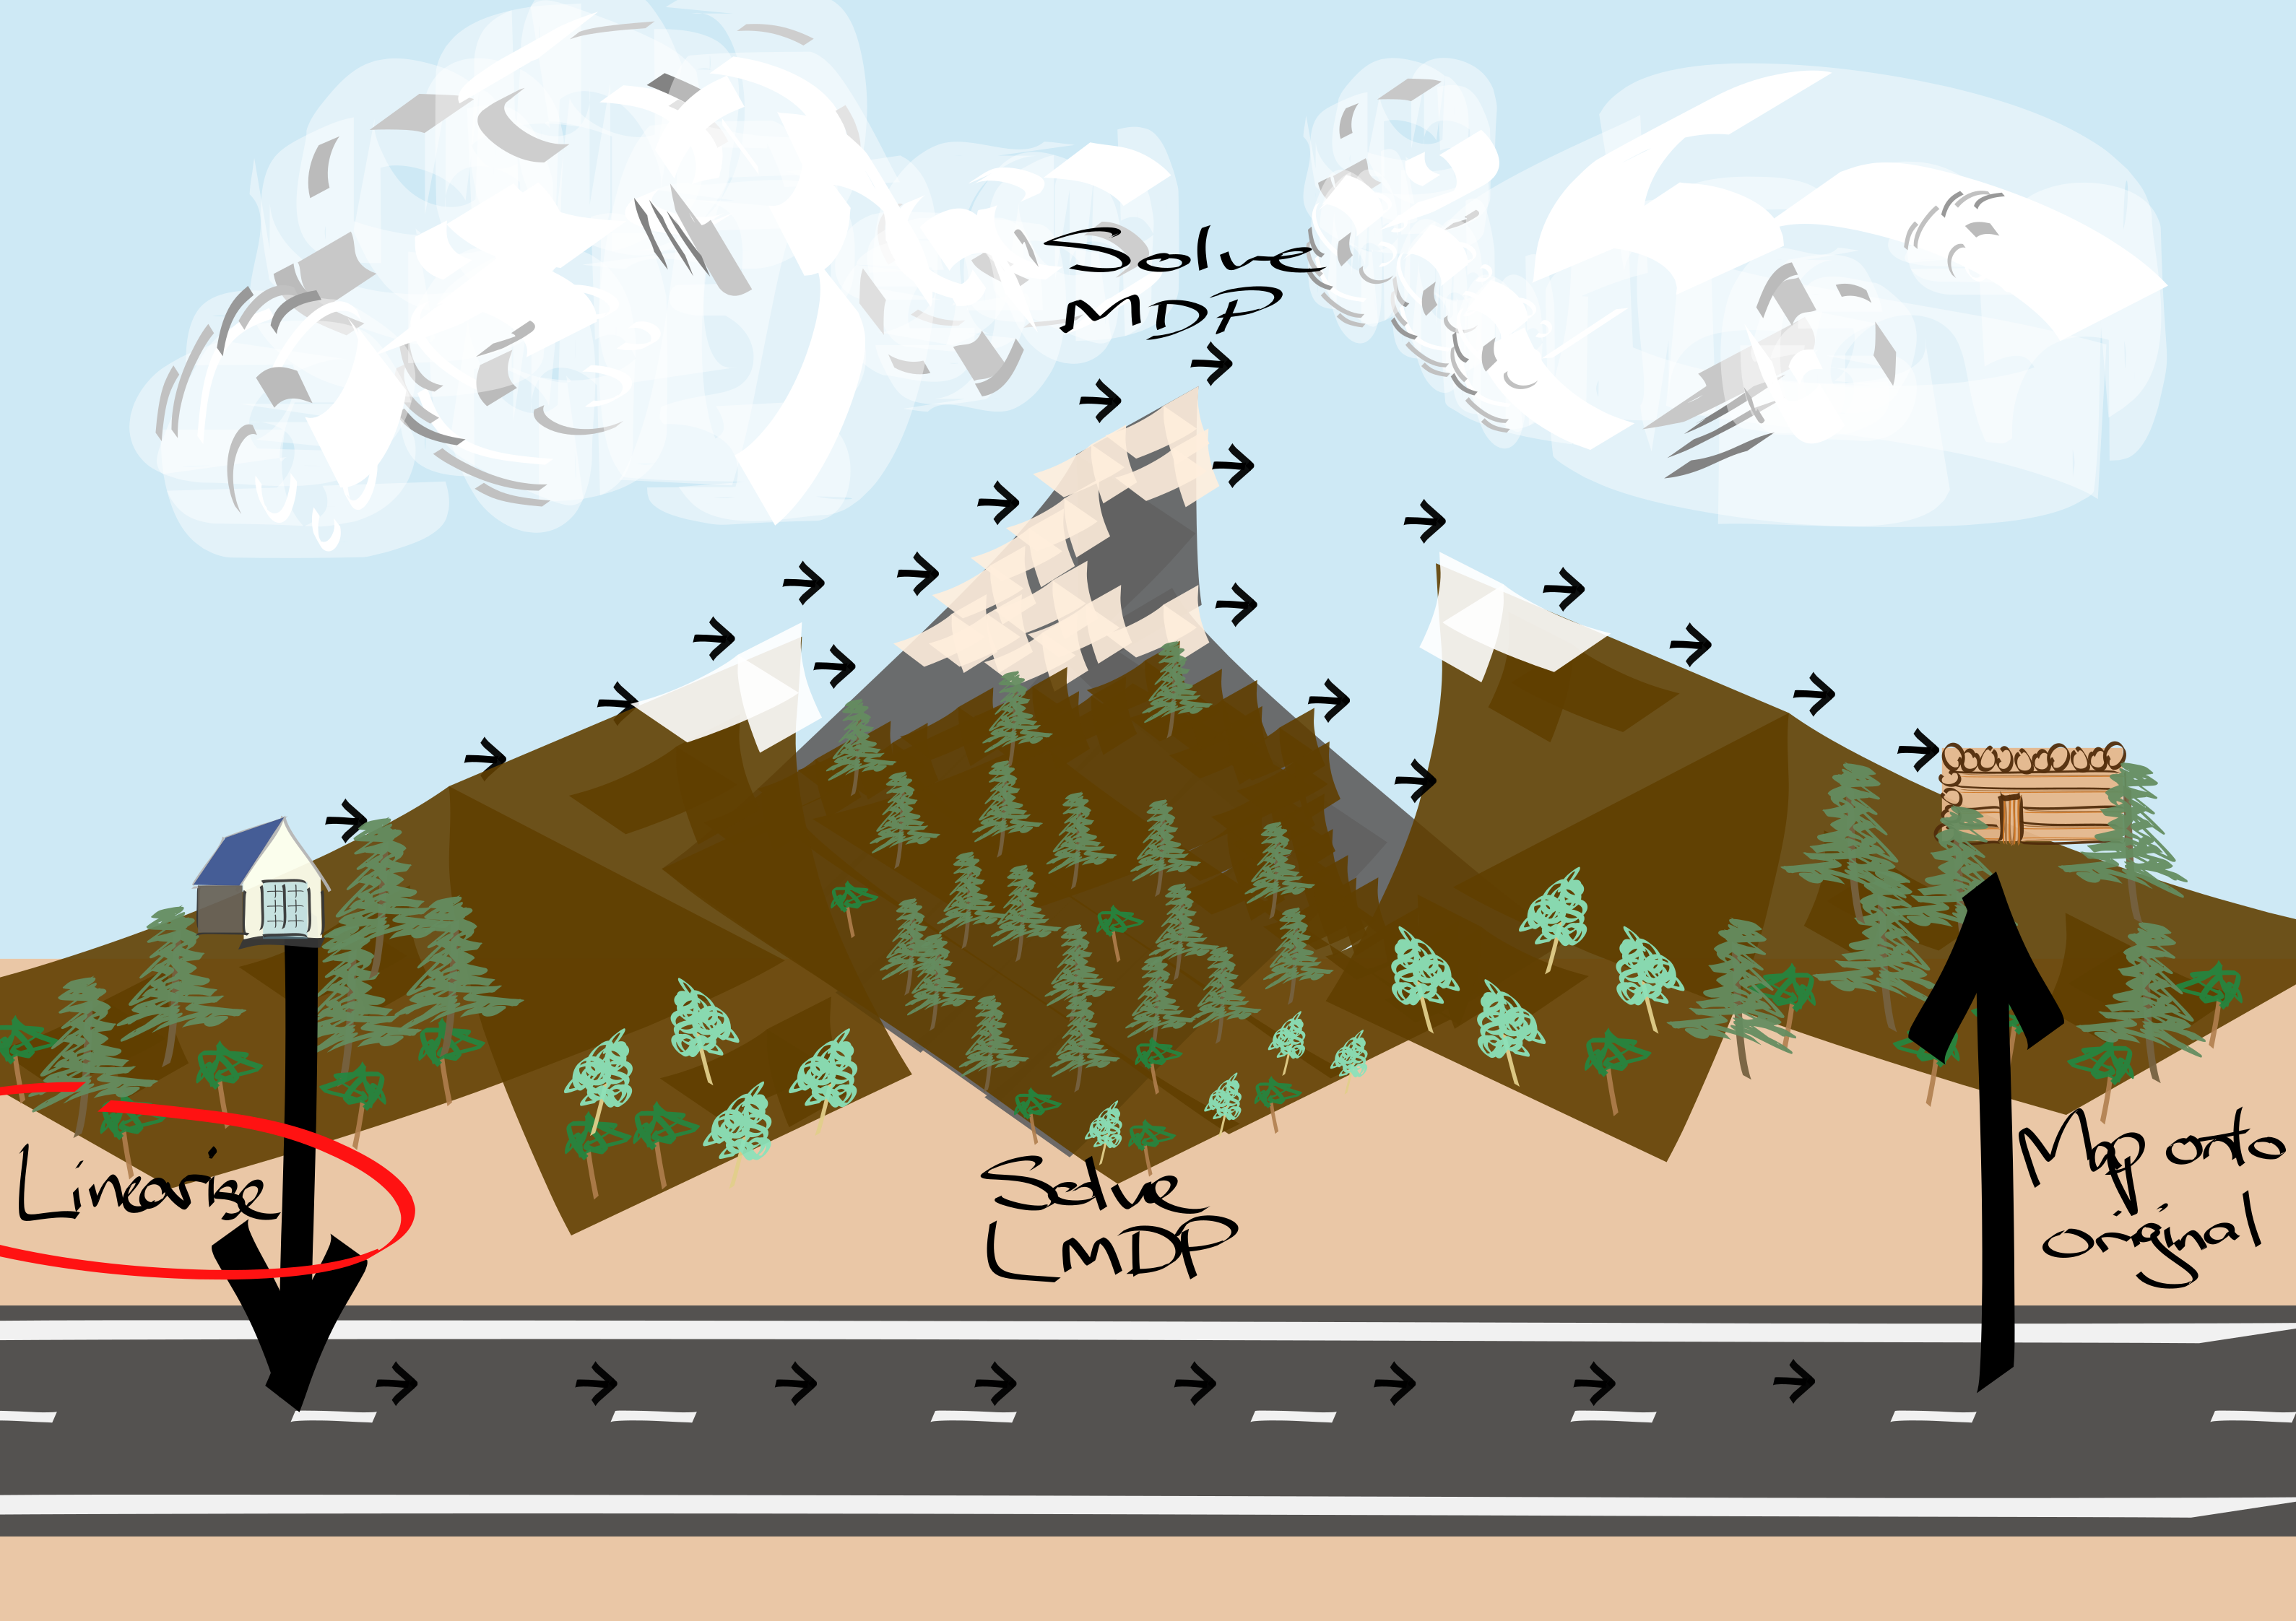
\includegraphics[width=0.6\textwidth,height=0.3\textheight]{../../pictures/drawings/abstract-representations-linear.png}
\caption{''}
\end{figure}

\begin{displayquote}
\textit{So, LMDPs can be easily solved. But how does solving LMDPs help us solve MDPs?}
\end{displayquote}

We want a way to transform a MDP into a LMDP, while preserving the
`structure' of the original MDP. But what do we mean by a MDP's structure?
The LMDP should; be able to represent the same transition dynamics as the original MDP (1),
and give the the same rewards was the original MDP (2). \cite{Todorov} {\color{red}(why? / intuition?!)}

\begin{align*}
\forall s, s' \in S, \forall a \in A, \exists u_a& \;\;\text{such that;} \\
P(s' | s, a) &= u_a(s'|s)p(s'|s) \tag{1} \\
r(s, a) &= q(s) - \text{KL}(P(\cdot | s, a) \parallel u_a(\cdot| s) ) \tag{2}
\end{align*}

% "We do not yet have theoretical error bounds but have found the approximation to be very accurate in practice" \cite{Todorov}

So, given a reward function, $r$, and a transition function, $P$,
from an MDP, we can use (1), (2) to solve for the unconditioned dynamics $p$ and a state reward $q$.
This transformation, from $P, r \to p, q$ requires $|S| \times |A|$ computations, as for each state in the
MDP \(|A|\) linear equations to solve. (For more explanation and a derivation see appendix [].)

However, are there some conditions that are missing?!
It might make sense to preserve the value of state-actions (3)? {\color{red}Because?}
And it would definitely make sense to preserve the optimal policy (4)? {\color{red}Because?}

\begin{align*}
\forall s, s' \in S, \forall a \in A, \forall \pi \in \Pi \\
z_{u_{\pi}}(s) = e^{v_{\pi}(s)} \tag{3} \\
P(s'|s, a) \cdot \pi^{* }(a|s) = u^{* }(s'|s) \tag{4}
\end{align*}

Where $z_{u_{\pi}}$ is the value (as evaluted by the LMDP) of the control $u_{\pi}(s'|s) = P(s'|s, a) \cdot \pi(a|s)$.

Todorov hopes that (1), (2), will be sufficient to give (4). But he does not prove it.
This is problem that we will return to.

% If the optimal policy is not preserved by the transformation of MDP to LMDP then solving the

\subsection{Decoding the optimal LMDP policy}

\begin{figure}[h!]
\centering
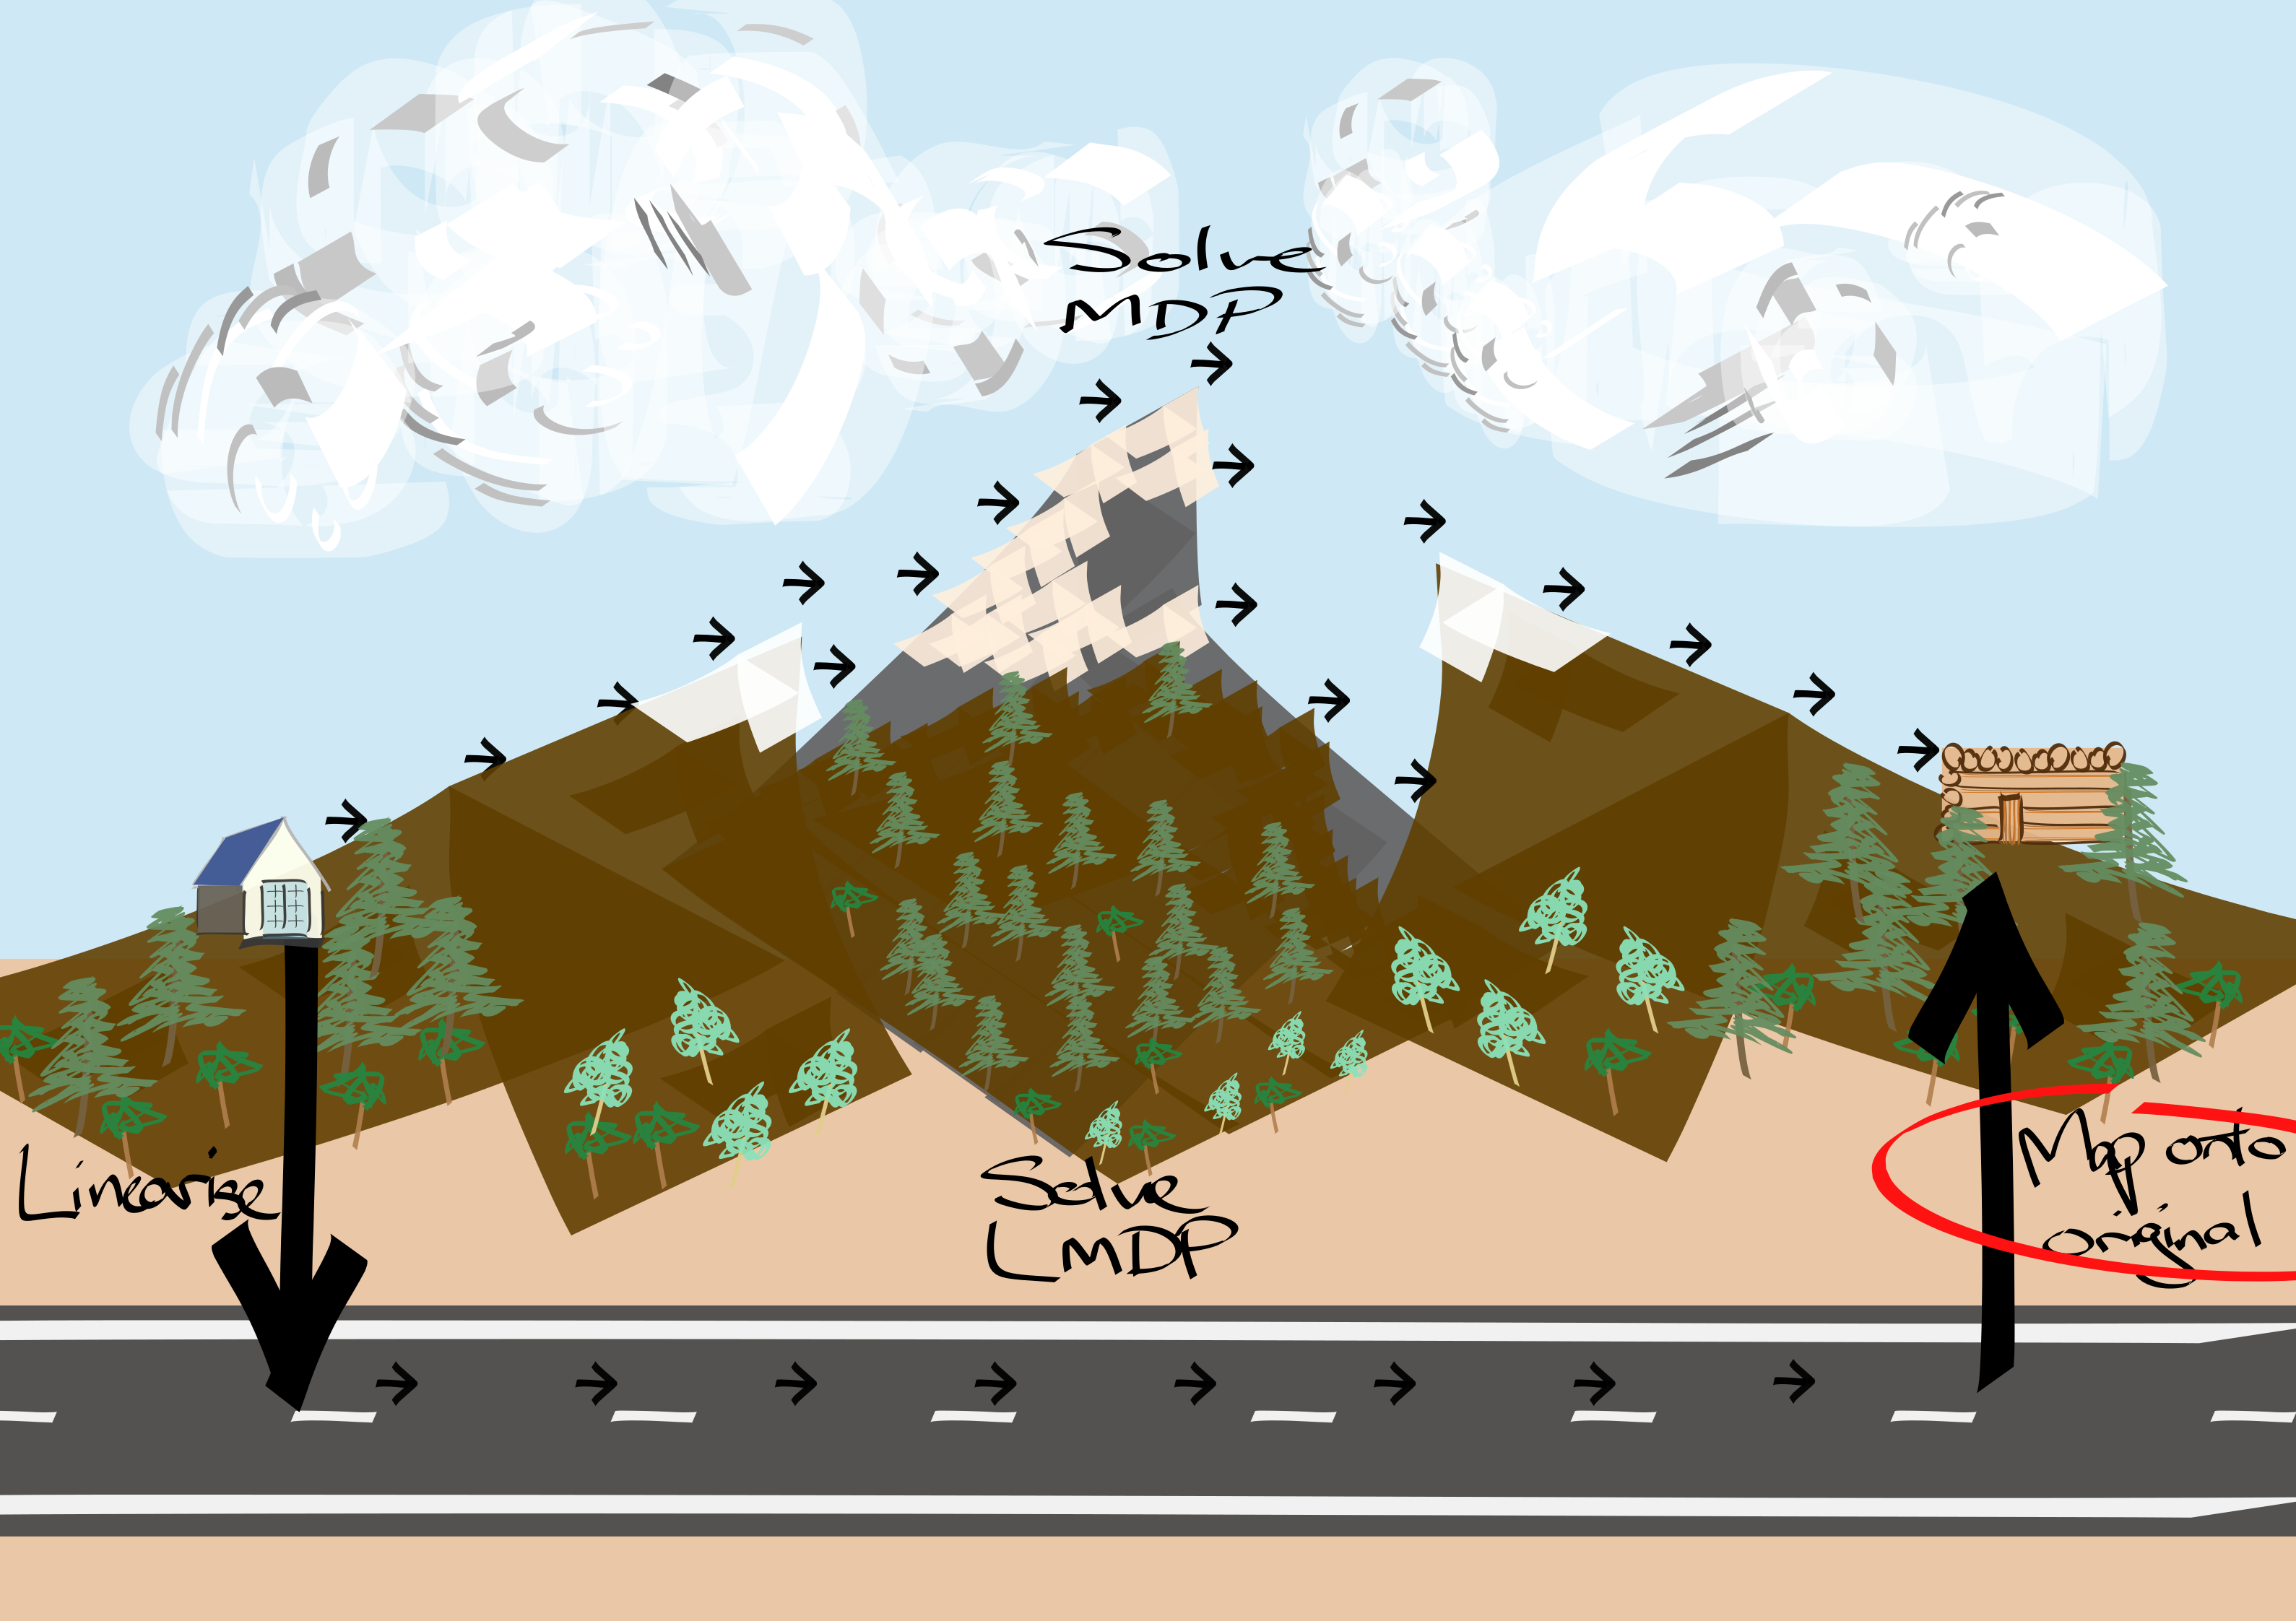
\includegraphics[width=0.6\textwidth,height=0.3\textheight]{../../pictures/drawings/abstract-representations-project.png}
\caption{''}
\end{figure}

\begin{displayquote}
\textit{How can we use the optimal control, $u^{* }$, to construct a policy that is optimal in the original MDP, $\pi_{u^* }$?}
\end{displayquote}

Here we get a glimpse at the structure of our abstraction.
The LMDP has disentangled the search for the optimal controls (solve the LMDP) (go to this or
that state) and the search for the optimal policy (how to actually
realise that control).

This decomposition is reminicent of goal conditioned approaches to heirarchical RL.
Where a higher level agent gives goals (go to this or that state) to a lower level
agent, who must figure out how to achieve that goal. \cite{Vezhnevets2017} {\color{red}more refs?!?}

This decomposition within the LMDP can be seen the optimal control decoding
step (currently being considered). We know which
states we want to be in, the $z^{* } / u^{* }$, from solving the LMDP, but,
we do not know how to implement those controls in the original MDP.
We can formulate this decoding problem as trying to match the optimal control (aka dynamics)
using the actions we have available.

\begin{align}
P_{\pi}(\cdot | s) = \sum_a P(\cdot | s, a) \pi(a | s) \\
\pi = \mathop{\text{argmin}}_{\pi} \text{KL}\Big(u(\cdot | s))\parallel P_{\pi}(\cdot | s)\Big)
\end{align}

{\color{red}TODO}

This optimisation problem has very little structure.
Maybe a way to add more structure?
But it's just a special type of matrix factorisation?!? Does it have a unique minima?

Maybe this isnt enough? Do we need to add a reward sensitive part as
well?!? (but what if the actual path we take to get there has a neg
rewards?!?)

It turns out that solving \textbf{P2} is asymptotically as hard as solving a MDP.
So nothing has been gained... (proof?!?)

Great. We have now built a way to solve a MDP with a LMDP. Does it work as hoped?

\subsubsection{Optimality of solutions via LMDPs}

\begin{quote}
\textit{Do these two paths lead to the same place?}
\end{quote}

One of the main questions we have not addressed yet is; if we solve the
MDP directly, or linearise, solve and project, do we end up in the same
place? This is a question about the completeness of our abstraction. Can
our abstraction represent (and find) the same solutions that the
original can? We can formalise this question as the difference between the optimal values or optimal policies.

\begin{align*}
\epsilon_{\pi} &= \text{KL}\Big(u(\cdot | s))\parallel P_{\pi}(\cdot | s)\Big) \\
\epsilon_{V} &= \parallel V_{\pi^{* }} - V_{\pi_{u^{* }}} \parallel_{\infty}
\end{align*}

{\color{red}Note!!!: $\epsilon_{\pi}$ isnt reliable. we have not preserved the values.
and therefore, there exist MDPs where the bellman equation is broken, meaning n some cases we cannot learn.}

Where $\epsilon_{\pi}$ will tell us if the optimal behaviours are different. But What we really care about
is whether their value is different. We might not care if the optimal control
yields a policy that is different from the optimal policy, as long as the
policy via optimal control achieves high performance. We can measure this with $\epsilon_{V}$.

To evaluate $V_{\pi_{u^{* }}}$, the value of the decoded optimal control, we can
set $P_{\pi} = u^{* }$. And solve $V = (I - \gamma P_{\pi})^{-1} \cdot r_{\pi}$.
However, $r_{u^{* }}$ doesnt really make sense as the reward is action
dependent. We would like to be able to calculate $r_{\pi_{u^{* } }}$, but we dont
explicity know \(\pi_{u^{* }}\). By solving $(I - \gamma P_{\pi^{* }})^{-1} \dot r$
we get the state-action values, or $Q$ values of the optimal control.

Results... Bad.

\begin{figure}
\centering
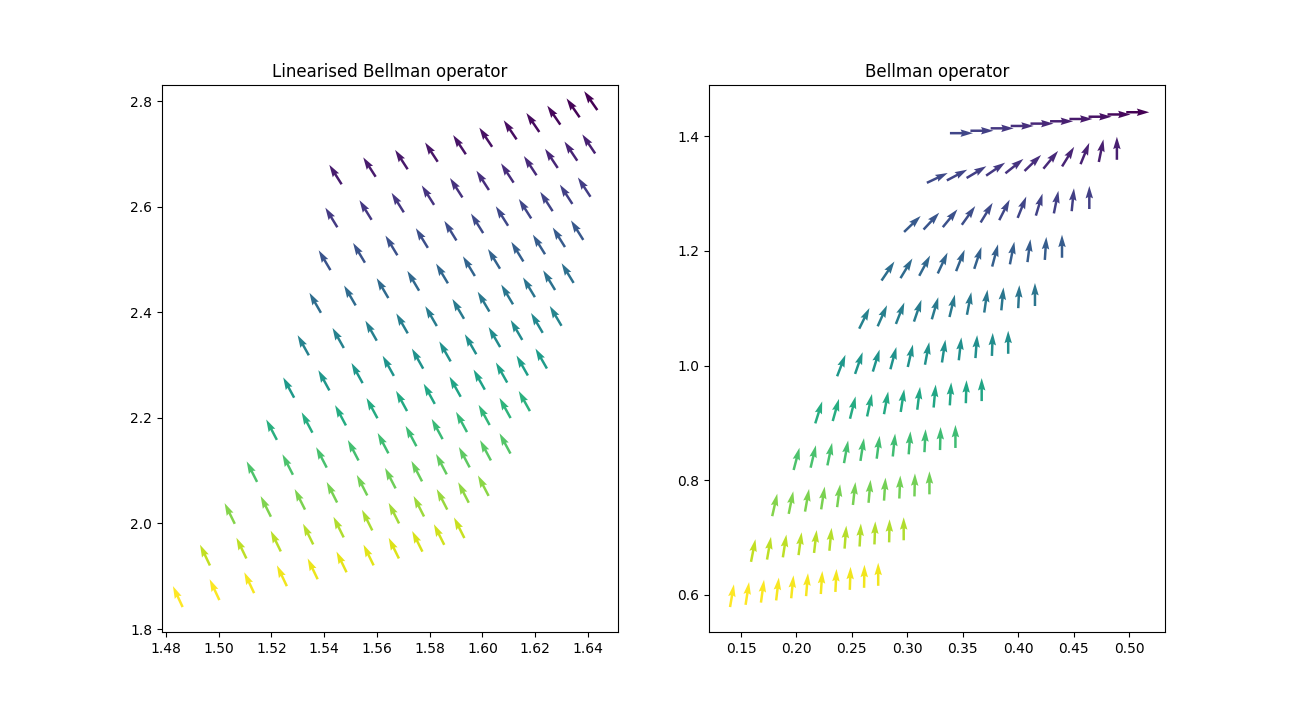
\includegraphics[width=0.75\textwidth,height=0.5\textheight]{../../pictures/figures/LBO_BO.png}
\caption{For the same MDP, shown is a comparison of the linear temporal difference operator (left), versus the true, Bellman, temporal difference operator (right). As expected, the Bellman temporal difference operator points towards the optimal value. But, ther linear temporal difference operator points elsewhere...}
\end{figure}

\begin{figure}
\centering
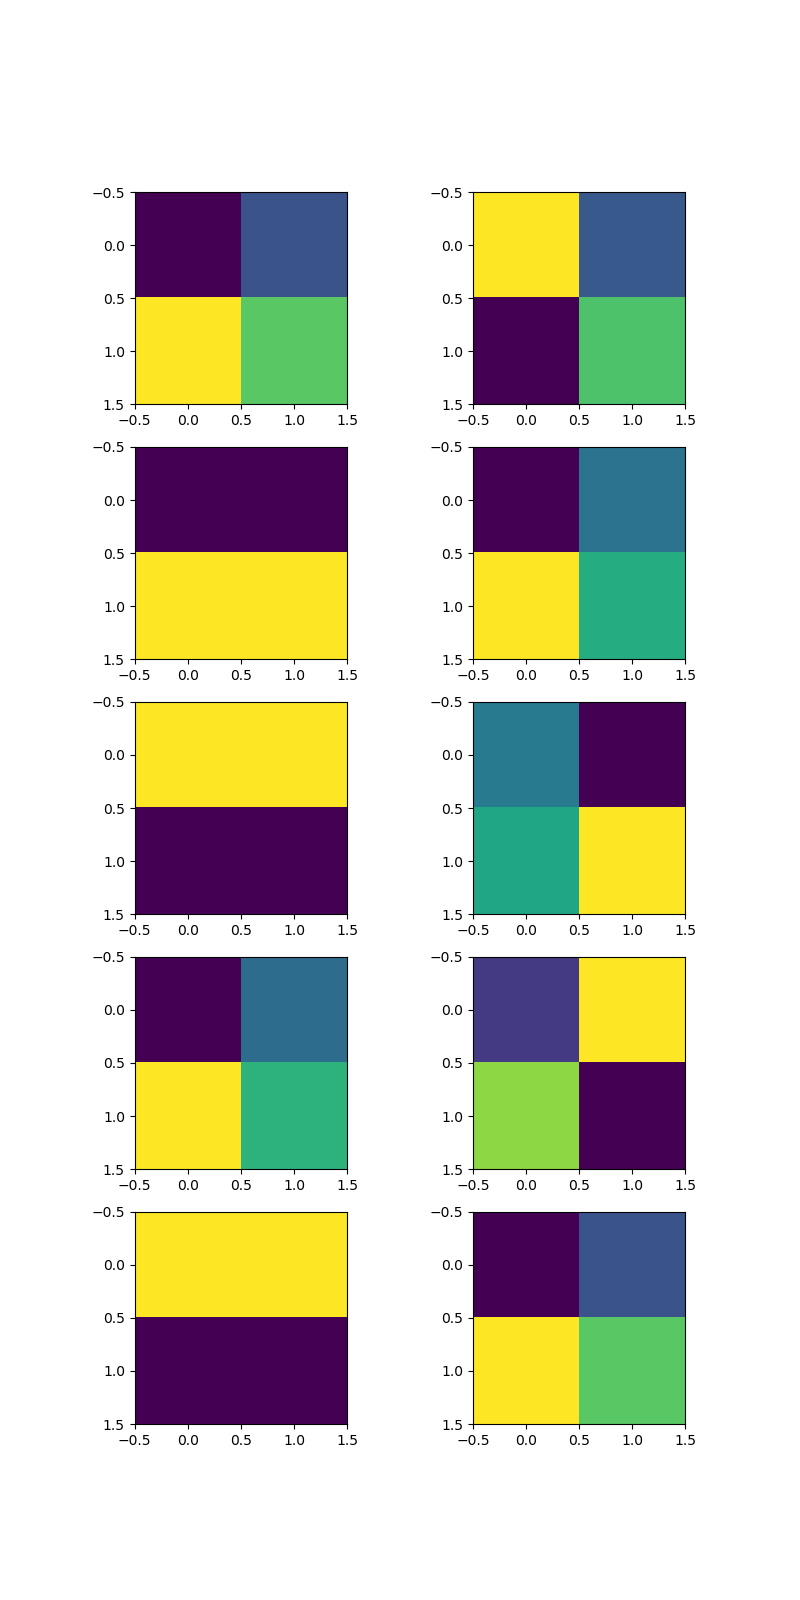
\includegraphics[width=0.5\textwidth,height=0.75\textheight]{../../pictures/figures/lmdp_mdp_optimal_dynamics.png}
\caption{A comparison between the optimal control (LMDP) and the optimal policy (MDP).}
\end{figure}

{\color{red}also include some numbers of the value error}

\subsection{Discussion}

\subsubsection{Validation} \label{lmdp-validation}

Unfortunately, Todorov \cite{Todorov2006,Todorov2009} never actually produced
any experiments that use the linear bellman equation to solve an MDP.
His experiments were with $Z$-learning, the linearised counterpart to $Q$-learning:

\begin{align*}
\tilde z(s) = e^{q(s)}z(s{'})^{\gamma} \tag{linearised bellman eqn}\\
z_{t+1}(s_i) = (1- \eta)z_{t}(s_i) + \eta\tilde z(s_i) \tag{$Z$ iteration}\\
\end{align*}

They make this work by hand picking $q$ so that the optimisation will converge to the optimal value.
Then they evaluate the accuacy of the value estimates.
They do not give a general way of constructing $q$ from a MDP.
Nor do they give an efficient way to map an optimal control to an optimal policy.
To understand the importance of these see the figures below.

\begin{figure}
\centering
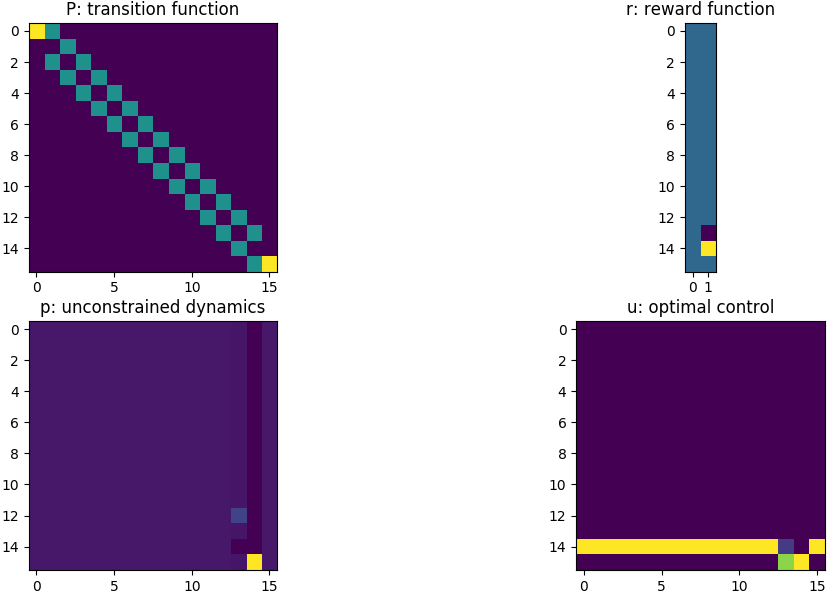
\includegraphics[width=0.7\textwidth,height=0.35\textheight]{../../pictures/figures/chain-test-zero-rewards.png}
\caption{A chain problem with zero reward on all states except the last two. A small negative reward, then a large positive one.
The optimal control to this problem is not sensible: in every state, jump to the state with positive reward.
It is not possible to make those transitions.}
\end{figure}

\begin{figure}
\centering
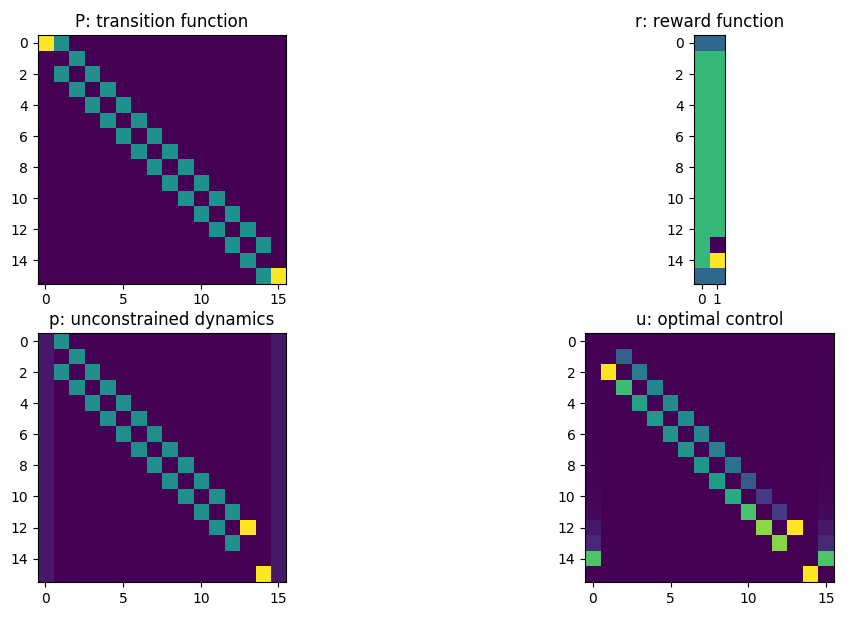
\includegraphics[width=0.7\textwidth,height=0.35\textheight]{../../pictures/figures/chain-test-pos-rewards.png}
\caption{A chain problem with positive rewards applied to all states.
Now the structure of the transition function has made it into the optimal control!
The LMDP's control can be decoded into a policy.}
\end{figure}

% \begin{figure}
% \centering
% 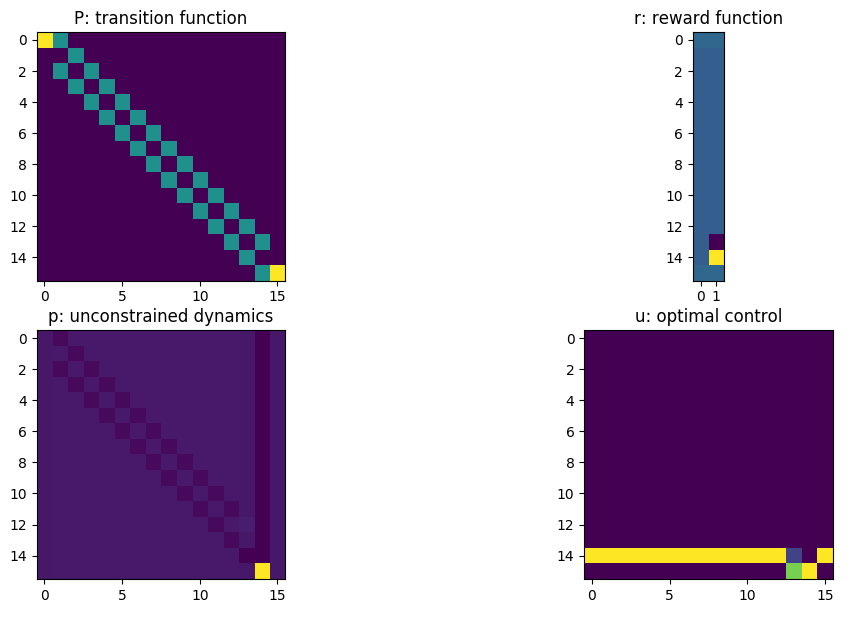
\includegraphics[width=1\textwidth,height=0.35\textheight]{../../pictures/figures/chain-test-neg-rewards.png}
% \caption{A chain problem with negative rewards applied to all states.
% Again, the structure of the transition function is missing.}
% \end{figure}

Because, there are no benchmarks that we can validate our implementation on,
there is some doubt about whether I implemented the LMDP correctly. While the
LDMP solution strategy, does occasionally pick the correct optimal policy, more often than not,
it gets it wrong.

\newpage

\subsubsection{Linearity in MDPs}

Todorov's formulation of LMDPs do not seem to allow you to reliably embed a MDP in a LMDP.
Despite this, it might still be possible to construct a linear MDP given different assumptions.

Let's reconsider Jin et al.'s approach \cite{Wang}. Construct a MDP where the value is a
linear function of a state-action representation and of a policy embedding.
To actually optimise this, we are required to use the bellman equation.
Not every (policy) embedding can be realised as a policy, so to constrain the search dynamics properly
we must use the bellman equation.

And this captures the essence of the problem. The Bellman equation is not linear.
We can linearise a MDP, but we will lose the ability to use the Bellman equation
to guide the search for the optimal policy.

% It seems that the main advantage gained by adding linearity in this way \cite{Wang} is the ease of analysis.
% Whether this type of linear abstraction actually reduces the sample or computational complexity has yet to be proved.


% Refs \cite{Todorov2006,Todorov2009,Zhong,Zhonga,Dvijotham,Wozabal}
% Linearise around the optimal policy. But how does that tell us how to act when not at the optimal policy?
